\chapter{Methodology}

Exclusively open-source resources have been used to carry out the thesis work. 
In particular, the orbital scenarios under examination have been simulated through dynamic propagation models created in Python, taking advantage of existing free Python libraries.   
In order to validate the results, the \textit{General Mission Analysis Tool} (GMAT) has been chosen as the reference software to make comparisons.
Even space debris mitigation has been performed thanks to the availability of an open-source software, DRAMA, published by ESA.

In the following paragraphs a brief description of the tools mentioned previously is presented.

\section{Python for Astrodynamics Applications}

Due to the computationally intensive nature of astrodynamics tasks, astrodynamicists have relied on compiled programming languages such as Fortran for the development of astrodynamics software.
Interpreted languages like Python on the other hand offer higher flexibility and development speed thereby increasing the productivity of the programmer.
While interpreted languages are generally slower than compiled languages, recent developments such as just-in-time (JIT) compilers or transpilers have been able to close this speed gap significantly. 
Another important factor for the usefulness of a programming language is its wider ecosystem which consists of the available open-source packages and development tools including integrated development environments and debuggers. 

In light of the above, Python can be considered as a suitable language for scientific computing due to the existence of well established libraries like NumPy and SciPy for mathematical calculations.
Not only do these libraries make use of compiled code from existing accelerated libraries, but it is also possible in Python to interface with compiled code to speed up specific algorithms where required.
This allows a user to define a problem in Python, while benefiting from the speed of compiled languages for computationally expensive algorithms.
Indeed, JIT-compiled dynamic languages such as Python with Numba have reached a competitive level of performance while still offering the advantages of lower complexity and better programmer productivity
\cite{eichhorn2018comparative}.

And not for nothing, nowadays, by a wide margin, Python is the most popular interpreted language in astronomy
\cite{momcheva2015software}.

\subsection{Numba}
Arguably, the most important library in the scientific Python stack is NumPy, which implements n-dimensional arrays and its related methods in C programming language, and wraps them using the CPython API (Application Programming interface).
It is a fundamental piece of software that powers most numerical codes written in Python nowadays.
However, while it is possible to vectorize certain kinds of numerical operations, there might be other cases where this may not be feasible and where the dynamic nature of Python leads to a performance penalty, especially when the algorithm involves several levels of nested looping.
To overcome these limitations it is possible to use Numba, an open-source library which can infer types for array-oriented and math-heavy Python code and generate optimized machine instructions using the LLVM compiler infrastructure
\cite{rodriguez2016poliastro}.
In brief, Numba is a JIT compiler for scientific Python, which allows to optimize the running time.

\subsection{poliastro}
\texttt{poliastro} is an open-source Python library for astrodynamics and orbital mechanics released under the MIT (Massachusetts Institute of Technology) license.
It features algorithms which are written in pure Python and compiled using Numba.
It is dedicated to astrodynamics applications, such as orbit propagation, resolution of the Kepler and Lambert problems, conversion between position and velocity vectors and classical orbital elements and orbit plotting
\cite{rodriguez2016poliastro}.
In addition, thanks to Astropy, poliastro can perform seamless coordinate frame conversions and use proper physical units and timescales.
At the moment, poliastro is the longest-lived Python library for astrodynamics, has contributors from all around the world, and several New Space companies and people in academia use it
\cite{rodriguez2022poliastro}.

\section{General Mission Analysis Tool}
The General Mission Analysis Tool is a software system for trajectory optimization, mission analysis, trajectory estimation, and prediction developed by NASA (National Aeronautics and Space Administration), the Air Force Research Lab, and private industry.
GMAT is designed to model, optimize, and estimate spacecraft trajectories in flight regimes ranging from LEO to lunar applications, interplanetary trajectories, and other deep space missions.
GMAT's design and implementation are based on four basic principles: open-source visibility for both the source code and design documentation; platform independence; modular design; and user extensibility
\cite{conway2010general}.

\section{Debris Risk Assessment and Mitigation Analysis} \label{drama_section}
The \textit{Debris Risk Assessment and Mitigation Analysis} software tool supports space missions in the analysis of every kind of debris related problems.
It is provided with the necessary computational and data reference by another tool: MASTER (\textit{Meteoroid and Space Debris Terrestrial Environment Reference}).
DRAMA includes five individual components, aiming at  aiding the verification of the compliance of space missions with mitigation guidelines and standards, like that ones mentioned in subsection \ref{space_debris_mitigation} \cite{braun2013drama}.

The first one is the \textit{Assessment of Risk Event Statistics} (ARES) tool which evaluates the annual rates of close approaches between an operational satellite of interest and debris in Earth orbits along with statistics on the necessary number of collision avoidance maneuvers and related $\Delta V$ and propellant mass.

The \textit{MASTER-based Impact flux and Damage Assessment Software} (MIDAS) assists the assessment of debris and meteoroid impact rates over the satellite's lifetime.

DRAMA also provides the estimation of the orbital lifetime and the evaluation of different possible disposal strategies after the End-of-Life (EOL) thanks to the \textit{Orbital SpaceCraft Active Removal} (OSCAR) tool.

The \textit{re-entry Survival And Risk Analysis} (SARA) tool allows the assessment of the re-entry survivability of all the different spacecraft components. 
It then provides the combined on-ground casualty risk given a world population model and the impact footprint of the surviving fragments.  

Finally, the \textit{Cross-section of Complex bodies} (CROC) intends to compute the cross-sectional areas of complex satellites and different possible attitudes laws after the EOL \cite{braun2020drama}.

% Figure \ref{drama_main_windo_fig} shows the main window of DRAMA software.
% \begin{figure}[h]
%     \centering
%     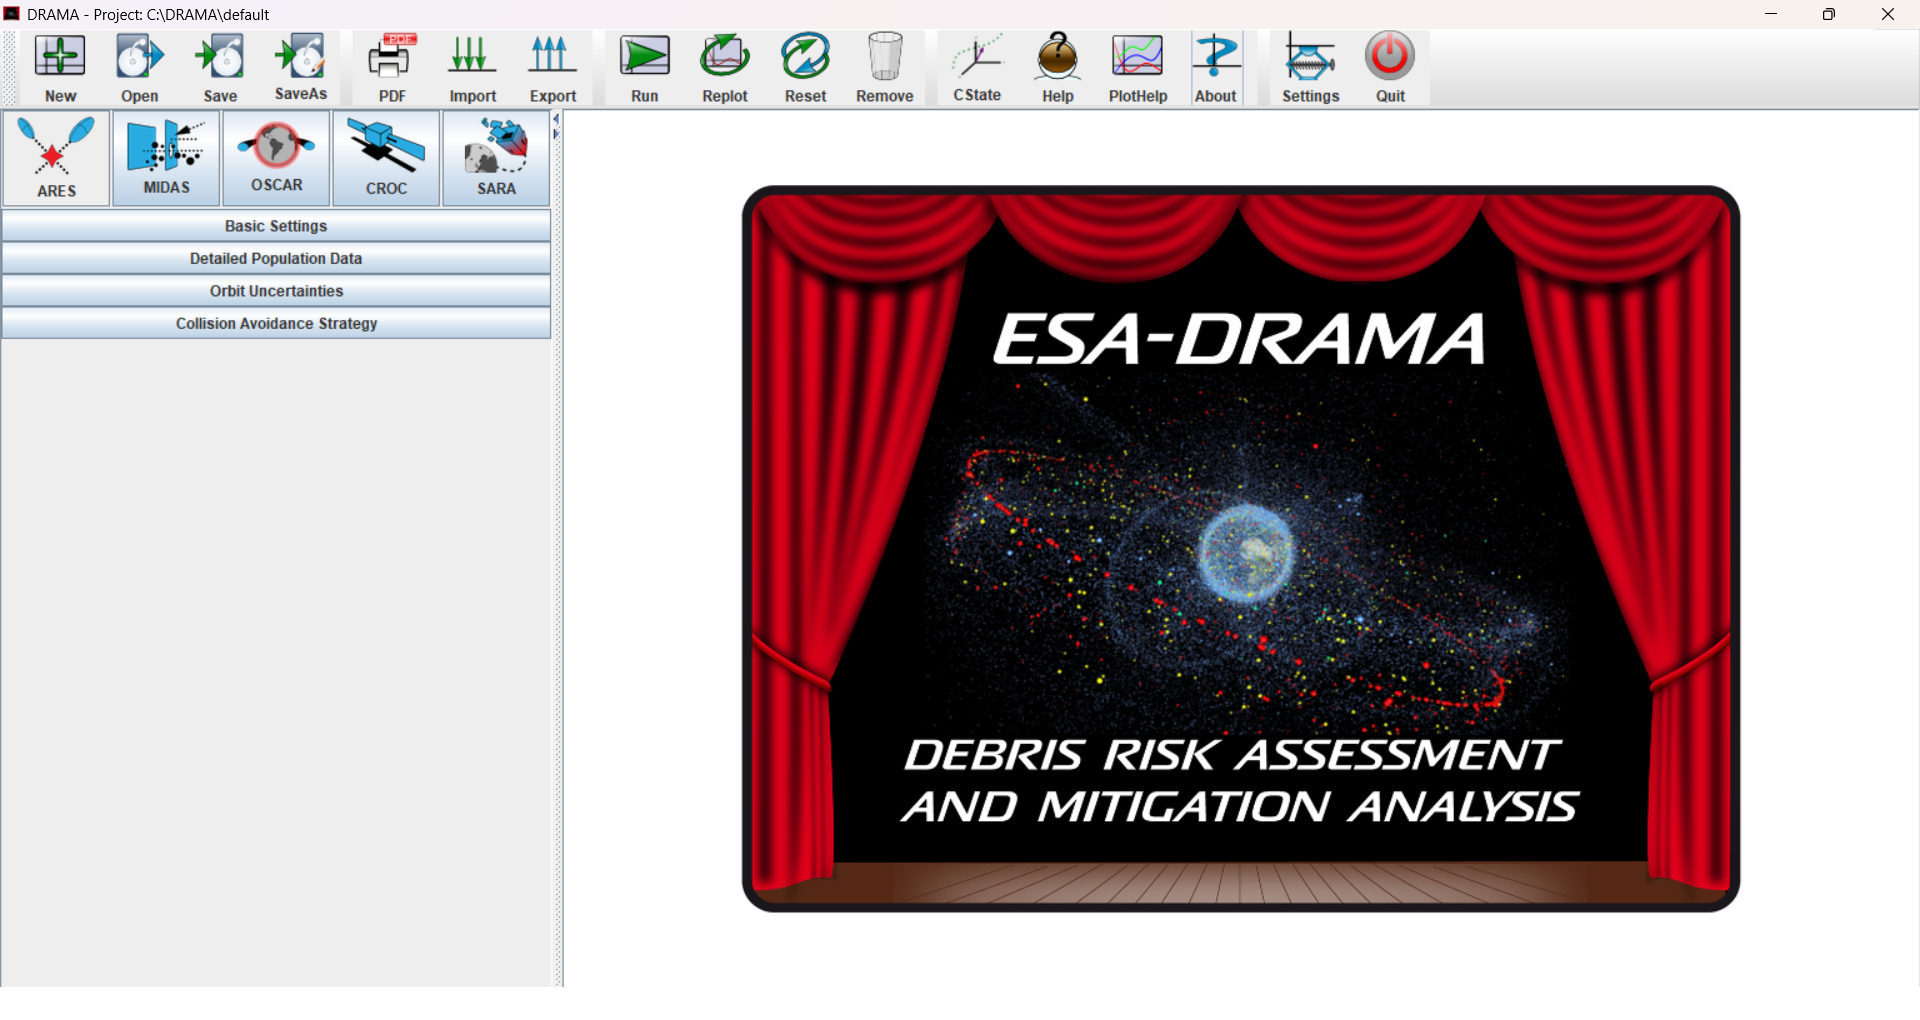
\includegraphics[scale=0.25]{img/drama_mainwindow.png}
%     \caption{Main window of DRAMA}
%     \label{drama_main_window_fig}
% \end{figure}